\documentclass{article}

\PassOptionsToPackage{numbers}{natbib}
\usepackage[dblblindworkshop]{neurips_2026}
\workshoptitle{Foundations of Language Model Security}

\usepackage[utf8]{inputenc}
\usepackage[T1]{fontenc}
\usepackage{url}
\usepackage{amsmath,amssymb,amsthm}
\usepackage{booktabs}
\usepackage{enumitem}
\usepackage{microtype}
\usepackage{xcolor}
\usepackage{tikz}
\usetikzlibrary{positioning,arrows.meta,fit,shapes.geometric,calc}
\usepackage{hyperref}

\newtheorem{definition}{Definition}
\newtheorem{theorem}{Theorem}
\newtheorem{corollary}{Corollary}


\title{Influence Tracking for Secure LLM Agents:\\
Preventing Privilege Escalation Under Worst-Case Model Behaviour}

\author{
  Anonymous Author(s)
}

\begin{document}
\maketitle

\begin{abstract}
Large language model (LLM) agents increasingly perform externally visible
actions on behalf of users. These agents process inputs originating from
multiple principals, creating security challenges that extend beyond
traditional access control. Existing defences primarily seek to prevent prompt
injection by improving model robustness, but such approaches remain dependent
upon empirical model behaviour and adaptive attack strategies.

This paper instead considers privilege escalation as the fundamental
system-level security objective for LLM agents. Prompt injection is treated as
one mechanism by which privilege escalation may occur, rather than the security
objective itself. We introduce \emph{Influence Tracking with Extrapolated
Security} (ITES), a provenance-based defence that derives the effective
authority of each execution directly from an existing access-control system.
ITES's authority-attenuation rule follows a low-water-mark intuition
structurally analogous to classical Biba integrity. We prove that authority is
monotonically non-increasing as influence accumulates, implying that
privilege escalation is impossible under the stated threat model.

To evaluate implementations of system-level defences, we introduce the
\emph{System-Level Evaluator for Defences} (SLED), which models executions
under worst-case language-model behaviour and exhaustively explores the
resulting system state space. Across approximately 1.5 million explored
execution traces, no successful privilege escalation or
information-exfiltration violations were observed, while maximal utility was
preserved for all tasks already authorised by the underlying access-control
system. We additionally report preliminary results from SLED-V, an exploratory
verification extension using solver-backed bounded model checking, which
detects seeded monitor defects and reveals that several published defence
abstractions satisfy their own properties while violating PE.
\end{abstract}

%% ------------------------------------------------------------------
\section{Introduction}
\label{sec:intro}

LLM agents are increasingly deployed as autonomous agents that read documents,
invoke tools, and perform externally visible actions on behalf of users. Unlike
traditional software, these agents operate over natural-language inputs
originating from multiple principals---users, documents, databases, APIs, and
other systems. Consequently, arbitrary information may influence decisions with
real-world consequences.

Prompt injection has emerged as a fundamental security challenge
\citep{rossi2024earlycategorizationpromptinjection}. An attacker may supply
carefully crafted instructions through any input channel, causing an agent to
ignore its intended behaviour. Although considerable progress has been made on
model-level defences
\citep{struq2024,spotlighting2024,chen2025defendingpromptinjectiondefensivetokens,chen2025secalign,liu2025datasentinel},
these approaches ultimately rely on the language model recognising or resisting
malicious instructions. Because prompt injection is inherently adaptive, such
defences cannot provide stable guarantees
\citep{pasquini2024neuralexec,choudhary2025detect,shao2025poisoning,yang2025checkpointgcg,jia2025criticalevaluation}.

This paper studies privilege escalation as the fundamental system-level
security problem for LLM agents \citep{provos2003preventing,davi2010privilege}.
Prompt injection is one mechanism by which privilege escalation may occur, but
it is not the only one. Since a system-level defence cannot generally prevent
arbitrary prompt injection without preventing the agent from processing
untrusted information, we focus instead on preventing any source of
influence from increasing authority. Under a worst-case threat model, the
relevant question is not whether an input is malicious, but whether every
principal influencing an action is authorised to perform that action.

Motivated by this observation, we introduce \emph{Influence Tracking with
Extrapolated Security} (ITES), a provenance-based enforcement mechanism in
which every execution inherits the effective authority implied by the
provenance of its inputs. We also introduce the \emph{System-Level Evaluator
for Defences} (SLED), which evaluates system-level defences independently of
language-model behaviour by exhaustively exploring the execution state space.
Across approximately 1.5 million explored execution traces, SLED observed no
successful privilege escalation or information exfiltration while preserving
maximal utility for all tasks consistent with the underlying access-control
system.

The principal contributions of this paper are:

\begin{enumerate}[leftmargin=*,nosep]
  \item We argue that privilege escalation, rather than prompt injection
    itself, is the appropriate system-level security objective for LLM agents
    (Section~\ref{sec:threat-model}).

  \item We introduce ITES, a provenance-based enforcement mechanism that
    computes effective authority from information provenance and existing
    access-control policies (Section~\ref{sec:ites}).

  \item We introduce SLED, an evaluation framework that exhaustively explores
    system behaviour under worst-case model assumptions
    (Section~\ref{sec:sled}).

  \item We report preliminary results from SLED-V, an exploratory verification
    extension using solver-backed bounded model checking
    (Section~\ref{sec:results-sledv}).
\end{enumerate}

The remainder of the paper is organised as follows.
Section~\ref{sec:related} discusses related work.
Section~\ref{sec:threat-model} defines the threat model and security objective.
Section~\ref{sec:ites} presents ITES and proves its security properties.
Section~\ref{sec:sled} introduces SLED. Section~\ref{sec:results} reports the
evaluation results. Section~\ref{sec:future} discusses future work, and
Section~\ref{sec:conclusion} concludes.

%% ------------------------------------------------------------------
\section{Related Work}
\label{sec:related}

Existing approaches to securing LLM agents can be broadly divided into
model-level defences, system-level defences, and evaluation frameworks.

\paragraph{Model-level defences.}
Model-level defences seek to make language models recognise or resist prompt
injection through improved prompting, alignment, fine-tuning, or auxiliary
models
\citep{struq2024,spotlighting2024,chen2025defendingpromptinjectiondefensivetokens,chen2025secalign,liu2025datasentinel}.
While often effective empirically, such methods necessarily depend upon the
behaviour of the underlying language model. Their security therefore remains
probabilistic: improvements in attack strategies or changes in model behaviour
may alter their effectiveness
\citep{pasquini2024neuralexec,choudhary2025detect,shao2025poisoning,yang2025checkpointgcg,jia2025criticalevaluation}.
By contrast, ITES assumes worst-case model behaviour and derives its security
guarantees entirely from system-level enforcement.

\paragraph{System-level defences.}
Several recent works address prompt injection through system-level enforcement
\citep{debenedetti2025defeatingpromptinjectionsdesign,wu2024systemleveldefenseindirectprompt,beurerkellner2025designpatternssecuringllm}.
The Dual LLM pattern separates planning from processing untrusted information
by employing a privileged planning model together with a quarantined parsing
model. CaMeL extends this with capability tracking and developer-defined
security policies enforced by a custom interpreter. Progent
\citep{progent2025} mediates tool calls with symbolic privilege-control
policies. PACT \citep{pact2026} tracks argument-level provenance. FORGE
\citep{forge2026} enforces history-sensitive Datalog policies. Each optimises
for a different security objective; our preliminary comparative verification
(Section~\ref{sec:results-sledv}) suggests that satisfying a defence-native
property does not imply PE safety.

ITES differs from these approaches by deriving authority directly from the
organisation's existing access-control system. Rather than introducing a
trusted planning model, binary trust classifications, or a new policy language,
ITES tracks the principals whose information influences each execution and
derives effective authority by intersecting their permissions. Consequently,
security depends only upon correct provenance tracking, access-control
enforcement, and the access-control system itself.

\paragraph{Classical integrity and information-flow control.}
ITES is inspired by information-flow tracking but differs in using provenance
to derive effective authority under an existing access-control system rather
than preventing information flows themselves. Biba \citep{biba1977} defines
integrity policies including low-water-mark variants; LOMAC
\citep{lomac2001} operationalises this in commodity operating systems.
Denning \citep{denning1976} provides the lattice model for secure information
flow; ITES's authority intersection is a meet in the powerset lattice over
permission sets. Goguen and Meseguer \citep{goguen1982} establish
noninterference, which is strictly stronger than the access-safety properties
verified here. Sabelfeld and Myers \citep{sabelfeld2003} and Myers and Liskov
\citep{myers1997difc} provide vocabulary for explicit and implicit flows and
decentralized IFC.

\paragraph{Evaluation.}
Most existing prompt-injection benchmarks evaluate a defence by measuring its
robustness against a fixed collection of attacks. AgentDojo
\citep{agentdojo2024} provides realistic prompt-injection tasks and metrics.
We treat such benchmarks as complementary: they test finite attack/defence
combinations, while SLED evaluates whether a defence satisfies its intended
property under arbitrary model behaviour.

Table~\ref{tab:comparison} compares representative approaches.

\begin{table}[t]
\centering
\small
\renewcommand{\arraystretch}{1.2}
\begin{tabular}{p{2cm}p{2.5cm}p{1.8cm}p{2cm}p{1.2cm}p{1.5cm}p{2cm}}
\toprule
\textbf{System} & \textbf{Security property} & \textbf{Provenance} &
\textbf{Authority source} & \textbf{Model trusted?} & \textbf{Policy lang.} &
\textbf{Verification} \\
\midrule
Model-level & PI resistance & N/A & Model & Yes & N/A & Benchmark \\
Dual-LLM & PI prevention & None & Isolation & Planner & None & None \\
CaMeL & Policy enforcement & Capabilities & Dev.\ policies & Planner & Custom & None \\
Progent & Privilege control & Arguments & Symbolic policy & Yes & Custom & None \\
PACT & Arg.\ provenance & Arguments & Provenance tags & Yes & Contracts & None \\
FORGE & Policy enforcement & History & Datalog policies & Yes & Datalog & None \\
ITES & PE prevention & Principals & Organisational ACS & \textbf{No} &
\textbf{Existing} & \textbf{SLED} \\
\bottomrule
\end{tabular}
\caption{Comparison of approaches to securing LLM agents. ITES is
distinguished by deriving authority from the existing ACS, not trusting the
model, and supporting verification.}
\label{tab:comparison}
\end{table}

%% ------------------------------------------------------------------
\section{Threat Model and Security Objective}
\label{sec:threat-model}

We consider an LLM-based agent that performs externally visible actions on
behalf of users. The agent receives information from multiple principals, both
directly through user prompts and indirectly through documents, retrieved
content, databases, APIs, and tool outputs. Any principal may provide arbitrary
inputs; ITES does not distinguish between malicious, misleading, or benign
cases.

We make no assumptions about the language model's ability to distinguish
instructions from data, identify malicious content, or resist prompt injection.
Instead, we adopt a worst-case threat model in which any information processed
by the model may arbitrarily influence subsequent executions. Here
``arbitrary'' means any well-typed proposal admitted by the system
interface---not malformed protocol behaviour, arbitrary code execution, or side
channels.

The enforcement mechanism, the access-control system (ACS), and the provenance
mechanism are assumed correct and uncompromised. Our threat model does not
consider denial-of-service, side-channel attacks, compromise of the enforcement
mechanism, incorrect access-control policies, or incorrect provenance
information.

\subsection{Access-Control System}

We model the access-control system as the tuple $(U, A, D, P, W, R)$
\citep{servos2017abac}, where $A$ is the set of externally visible
parameterised actions, $U$ is the set of principals, $D$ is the set of data
objects, $P \subseteq U \times A$ is the permission relation, $W \subseteq
D \times U$ specifies authorship, and $R \subseteq D \times U$ specifies read
access. For principal $u \in U$ and action $a \in A$, $P(u,a)$ holds iff $u$ is
authorised to perform $a$. Permissions are not assumed to be hierarchical.

\subsection{Security Objective}

Inspired by tracking privilege \citep{provos2003preventing,davi2010privilege},
the objective of ITES is to prevent privilege escalation rather than to prevent
prompt injection.

\begin{definition}[Influencing Principal]
\label{def:influence}
A principal $u$ influences an action if information originating from $u$
contributes, directly or indirectly, to the execution that produces the action.
The set of influencing principals for execution $e$ is denoted
$\mathrm{Influence}(e)$.
\end{definition}

\begin{definition}[Privilege Escalation]
\label{def:pe}
Privilege escalation occurs iff an action $a \in A$ is performed for which
there exists an influencing principal $u \in \mathrm{Influence}(e)$ satisfying
$\neg P(u,a)$.
\end{definition}

\subsection{Trusted Computing Base}

\begin{center}
\small
\begin{tabular}{p{0.28\linewidth}p{0.62\linewidth}}
\toprule
\textbf{Component} & \textbf{Role} \\
\midrule
Adversarial & LLM proposals, prompt/document/tool content, principals without
required permissions \\
\addlinespace
Trusted & Principal authentication, provenance attachment, policy decision
point, reference monitor / transition semantics, effect mediation \\
\addlinespace
Not proved & Provenance correctness, ACS correctness, unbounded deployment
security, arbitrary Python equivalence, provider isolation, subjective user
intent \\
\bottomrule
\end{tabular}
\end{center}

%% ------------------------------------------------------------------
\section{Influence Tracking with Extrapolated Security}
\label{sec:ites}

The central principle of ITES is that every execution inherits the effective
authority implied by the provenance of its inputs. Any action performed during
an execution is permitted only if every principal influencing that execution is
authorised to perform the action under the existing access-control system.

\begin{figure}[t]
\centering
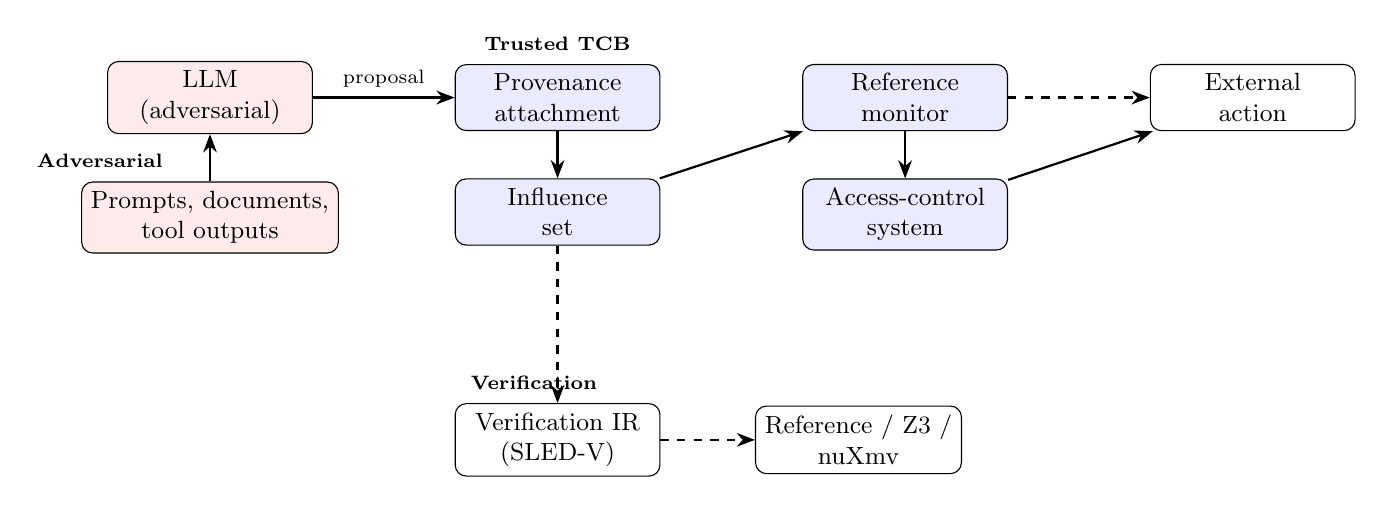
\begin{tikzpicture}[
  node distance=0.6cm and 1.2cm,
  every node/.style={font=\small},
  box/.style={draw, rounded corners, minimum height=0.8cm, minimum width=2.6cm, align=center, fill=white},
  adversarial/.style={draw, rounded corners, minimum height=0.8cm, minimum width=2.6cm, align=center, fill=red!8},
  trusted/.style={draw, rounded corners, minimum height=0.8cm, minimum width=2.6cm, align=center, fill=blue!8},
  arr/.style={-Stealth, thick},
  darr/.style={-Stealth, thick, dashed},
]
\node[adversarial] (llm) {LLM\\(adversarial)};
\node[adversarial, below=of llm] (inputs) {Prompts, documents,\\tool outputs};
\node[trusted, right=1.8cm of llm] (prov) {Provenance\\attachment};
\node[trusted, below=of prov] (context) {Influence\\set};
\node[trusted, right=1.8cm of prov] (monitor) {Reference\\monitor};
\node[trusted, below=of monitor] (acs) {Access-control\\system};
\node[box, right=1.8cm of monitor] (action) {External\\action};
\node[box, below=2.0cm of context] (ir) {Verification IR\\(SLED-V)};
\node[box, right=of ir] (solvers) {Reference / Z3 /\\nuXmv};

\draw[arr] (inputs) -- (llm);
\draw[arr] (llm) -- node[above,font=\scriptsize]{proposal} (prov);
\draw[arr] (prov) -- (context);
\draw[arr] (context) -- (monitor);
\draw[arr] (monitor) -- (acs);
\draw[arr] (acs) -- (action);
\draw[darr] (monitor) -- (action);
\draw[darr] (context) -- (ir);
\draw[darr] (ir) -- (solvers);

\node[font=\scriptsize, above=0.05cm of inputs, xshift=-1.4cm] {\textbf{Adversarial}};
\node[font=\scriptsize, above=0.05cm of prov] {\textbf{Trusted TCB}};
\node[font=\scriptsize, above=0.05cm of ir, xshift=-0.3cm] {\textbf{Verification}};
\end{tikzpicture}
\caption{ITES architecture. Adversarial components (red) supply arbitrary
inputs. The trusted computing base (blue) attaches provenance, computes the
influence set, and mediates actions through the ACS. SLED-V (dashed) verifies
a serialisable IR abstraction.}
\label{fig:architecture}
\end{figure}

\subsection{Influence Tracking}

The initial influence set of execution $e$ with inputs $ds \subseteq D$ is:
\[
\mathrm{Influence}(e) = \bigcup_{d \in ds} \{u \in U \mid W(d,u)\}
\]
Every object produced by an execution inherits the complete influence set of
that execution. Objects include intermediate LLM outputs, files, database
entries, and messages. Tool outputs are handled according to the
access-control system: trusted tools may produce objects associated with a
trusted system principal, whereas untrusted tools produce objects associated
with the principal on whose behalf the tool was invoked. Influence accumulates
monotonically throughout an execution chain; under the conservative provenance
model, influence is never removed.

\subsection{Authorisation}

Given execution $e$ with influence set $I = \mathrm{Influence}(e)$, ITES
permits action $a \in A$ iff:
\[
\mathrm{Allow}(I, a) \iff I \neq \varnothing \;\land\; \forall u \in I,\; P(u,a)
\]
The non-empty condition prevents vacuous authority. The effective authority is
$\mathrm{Permitted}(I) = \bigcap_{u \in I} \{a \in A \mid P(u,a)\}$. We
conservatively model an execution as reading every supplied input before
producing output; an execution may access datum $d$ only if $\forall u \in I,\;
R(d,u)$. This provides a straightforward confidentiality guarantee independent
of subsequent execution behaviour.

\subsection{Maximal Secure Authorisation}

The authorisation rule used by ITES is maximally permissive while preserving
the security objective of Section~\ref{sec:threat-model}.

\begin{theorem}[Maximal Secure Authorisation]
\label{thm:maximal}
ITES authorises the maximal set of actions that can be permitted without
allowing privilege escalation.
\end{theorem}

\begin{proof}
ITES authorises exactly $\mathrm{Permitted}(I)$. Suppose an alternative
authorisation rule permits a strict superset of this action set. Then there
exists an action $a \notin \mathrm{Permitted}(I)$ that the alternative rule
permits. Since $a \notin \mathrm{Permitted}(I)$, there exists an influencing
principal $u \in I$ such that $\neg P(u,a)$. Executing $a$ therefore satisfies
Definition~\ref{def:pe} and constitutes privilege escalation. Hence any
authorisation rule permitting a strict superset of the actions authorised by
ITES necessarily permits privilege escalation.
\end{proof}

\subsection{Authority Monotonicity}

A consequence of the authorisation rule is that additional influence can never
increase authority.

\begin{theorem}[Authority Monotonicity]
\label{thm:monotonicity}
For a fixed ACS state, if $\mathrm{Influence}(e_1) \subseteq
\mathrm{Influence}(e_2)$, then
$\mathrm{Permitted}(\mathrm{Influence}(e_2)) \subseteq
\mathrm{Permitted}(\mathrm{Influence}(e_1))$.
\end{theorem}

\begin{proof}
The effective authority of an execution is defined as the intersection of the
permissions possessed by its influencing principals. Adding additional
influencing principals introduces additional intersections but never removes
existing ones. Therefore the resulting permission set can only remain unchanged
or decrease.
\end{proof}

Authority therefore decreases monotonically throughout an execution chain. Once
a lower-authority principal influences a computation, no subsequent execution
derived from that computation can regain permissions removed by that influence.

\paragraph{Relationship to classical integrity.}
ITES follows a \emph{low-water-mark} intuition: incorporating additional,
potentially lower-authority influence cannot increase effective authority. This
is structurally analogous to Biba's low-water-mark integrity policy
\citep{biba1977}, operationalised in systems such as LOMAC
\citep{lomac2001}. The similarity is structural rather than an equivalence of
policy models. Low-water-mark integrity lowers a subject's effective integrity
after consuming lower-integrity information. ITES instead retains the
identities of all conservatively influencing principals and computes permitted
parameterised actions from the intersection of their current ACS permissions.
Attenuation is induced by organisational authority rather than by assigning a
single integrity label to the execution. When permission sets are ordered by
inclusion, intersection is their meet \citep{denning1976}.

\subsection{Security Guarantee}

The maximal secure authorisation and authority monotonicity theorems
immediately yield the principal security result.

\begin{corollary}
\label{cor:pe-prevention}
Under the threat model of Section~\ref{sec:threat-model}, and assuming correct
enforcement of influence tracking, provenance, and access-control checks,
ITES prevents privilege escalation.
\end{corollary}

\begin{proof}
By Theorem~\ref{thm:maximal}, ITES permits only actions that do not constitute
privilege escalation. Therefore every principal influencing $e$ is authorised
to perform $a$. By Definition~\ref{def:pe}, privilege escalation requires the
existence of an influencing principal lacking permission for the executed
action. Such a principal cannot exist if the action is permitted by ITES.
\end{proof}

This guarantee is independent of the source of influence. Prompt injection,
retrieved documents, compromised tools, and arbitrary model behaviour are
treated uniformly: once information contributes to an execution, the authority
of that execution is constrained by the permissions of the corresponding
principals. Consequently, ITES prevents privilege escalation regardless of how
the influence was introduced.

%% ------------------------------------------------------------------
\section{SLED: A System-Level Evaluator for Defences}
\label{sec:sled}

Existing evaluations of prompt-injection defences typically measure robustness
against a finite collection of attacks. Such evaluations are necessarily
incomplete: passing a benchmark demonstrates robustness only against the attacks
it contains. We instead evaluate whether a system-level defence correctly
enforces its intended security properties regardless of model behaviour.

\subsection{Worst-Case Model Behaviour}

SLED treats the language model as an adversarial component. Rather than
executing a particular model, each execution is a nondeterministic black box
that may produce any well-typed behaviour consistent with the system interface.
This corresponds directly to the threat model of
Section~\ref{sec:threat-model}. The resulting guarantees depend only on the
defence, the access-control system, and the assumed environment.

\subsection{State-Space Exploration}

SLED represents an agent as a sequence of executions connected through the
objects they consume and produce. Beginning from an initial state, SLED
repeatedly enumerates every action that may result from each pending execution.
Executing an action updates the environment, creates new objects, propagates
influence according to ITES, and may schedule further executions. Exploration
continues until every reachable state has been visited or a bound is reached.

SLED reports four verdicts:
\begin{description}[nosep,leftmargin=*]
\item[\textsc{SAFE}] The finite reachable state space was exhausted without
violation.
\item[\textsc{Bounded\_Safe}] No violation was found, but a configured bound
truncated work.
\item[\textsc{UNSAFE}] A safety property failed with a counterexample.
\item[\textsc{UNKNOWN}] Modelling, property, or adapter evaluation failed.
\end{description}

\subsection{Environment Models and Trace Classification}

SLED separates the evaluation algorithm from the environments being evaluated.
An environment specifies principals, the access-control system, available
data, and tools. Each explored trace is classified according to observable
system-level outcomes: security properties (privilege escalation, information
exfiltration, unauthorised actions) and utility (whether the intended task is
completed while respecting the access-control system). Classification is
independent of the internal behaviour of the language model.

\subsection{SLED-V: Exploratory Verification Extensions}
\label{sec:sledv}

SLED-V extends SLED with a serialisable verification IR that can be checked by
independent backends: a reference interpreter, Z3 bounded model checking, and
a nuXmv subset adapter. Properties include unauthorised execution, forbidden
observation, provenance monotonicity, and branch isolation. Property-scoped
cone-of-influence (COI) reduction removes irrelevant variables while preserving
verdicts and counterexample liftability. The IR is a hand-written abstraction
of the runtime kernel; formal equivalence is not claimed. Preliminary
verification results are reported in Section~\ref{sec:results-sledv}.

%% ------------------------------------------------------------------
\section{Results}
\label{sec:results}

We evaluated ITES using SLED across three representative organisational
environments. Each environment defined an access-control system, available
data, agent workflows, and task specifications, while SLED exhaustively
explored every execution trace consistent with the threat model of
Section~\ref{sec:threat-model}. Exploration was limited to a maximum recursive
execution depth of three. Across all environments, SLED explored approximately
1.5 million execution traces. Approximately 15\% of traces reached the
execution-depth bound and were excluded from subsequent analysis.

\begin{table}[h]
\centering
\begin{tabular}{lcc}
\hline
Environment & Explored Traces & Incomplete Traces\\
\hline
1 & 422\,535 & 40\,040\\
2 & 996\,451 & 159\,112\\
3 & 43\,621 & 19\,755\\
\hline
Total & 1\,462\,607 & 218\,907\\
\hline
\end{tabular}
\caption{Summary of exhaustive state-space exploration.}
\label{tab:exploration}
\end{table}

\subsection{Security}

\begin{table}[h]
\centering
\begin{tabular}{lccc}
\hline
Environment & Secure Goal Actions & Successful PE & Blocked PE\\
\hline
1 & 176\,352 & 0 & 352\,704\\
2 & 381\,328 & 0 & 878\,096\\
3 & 45\,488 & 0 & 28\,852\\
\hline
\end{tabular}
\caption{Action-level evaluation results. Every attempted privilege escalation
was blocked.}
\label{tab:action_results}
\end{table}

Across all explored traces, SLED observed no successful privilege escalation
and no successful information-exfiltration task. These observations are
consistent with the theoretical guarantees of Section~\ref{sec:ites}.

As a representative example, consider a workflow in which Alice authors a
confidential document and Bob subsequently requests that the agent email its
contents. The resulting execution inherits influence from both Alice and Bob.
Because Bob lacks permission to perform the requested action, the effective
authority excludes the email action, and the request is blocked.

\subsection{Utility}

\begin{table}[h]
\centering
\begin{tabular}{lccc}
\hline
Environment & Secure Tasks & Successful PE Tasks & Blocked PE Tasks\\
\hline
1 & 2\,118\,454 & 0 & 75\,648\\
2 & 4\,756\,190 & 0 & 107\,136\\
3 & 141\,342 & 0 & 0\\
\hline
\end{tabular}
\caption{Task-level evaluation results. Every secure task remained achievable.}
\label{tab:task_results}
\end{table}

ITES achieved maximal system-level utility: every task already authorised by
the access-control system remained executable, while every attempted privilege
escalation was correctly blocked. Several workflows that appear desirable
from a usability perspective are fundamentally incompatible with the underlying
access-control system because they require authority to increase during
execution. ITES exposes these as requiring explicit delegation or revised
organisational policy.

\subsection{Preliminary Verification Results (SLED-V)}
\label{sec:results-sledv}

We report preliminary SLED-V results on finite IR models. These are
exploratory, demonstrating the methodology on small models.

SLED-V detects all five native negative controls and 11 direction-readiness
mutants (7 delegation, 4 disclosure), each with one-step counterexamples
(Table~\ref{tab:defect-detection}). The reference interpreter, COI-reduced
model, and Z3 BMC agree on both safe and unsafe fixtures
(Table~\ref{tab:checker-agreement}). COI reduction removes irrelevant
variables while preserving verdicts, scaling to 16 noise variables without
change (Tables~\ref{tab:coi-reduction},~\ref{tab:coi-scaling}). Several
published defence abstractions satisfy their own properties while violating PE
(Table~\ref{tab:comparative-defence}), suggesting that satisfying a
defence-native property does not imply PE safety. This is a model-level
comparison, not an implementation-level evaluation.

% GENERATED FILE -- do not edit by hand.
% Source: research\output\runs\native-sled-reproduction-v1\result.json; research\output\runs\direction-readiness-v1\security-mutations.json
% SHA-256: 37eacfc1e8002d724ff0deeeaef23fc435cbb5cab47dfecbbba8cd43f0200a2c
% Run: python scripts/generate_flmsec_tables.py
\begin{table}[t]
\centering
\small
\begin{tabular}{p{4cm}cc}
\toprule
\textbf{Defective monitor} & \textbf{Detected} & \textbf{Witness length} \\
\midrule
no\_defence & \checkmark & 1 \\
union\_permissions & \checkmark & 1 \\
initiator\_only & \checkmark & 1 \\
latest\_input\_only & \checkmark & 1 \\
no\_read\_check & \checkmark & 1 \\
delegation/widened\_scope & \checkmark & 1 \footnotesize(delegation\_attenuated) \\
delegation/wrong\_beneficiary & \checkmark & 1 \footnotesize(delegation\_beneficiary\_bound) \\
delegation/reuse & \checkmark & 1 \footnotesize(delegation\_single\_use) \\
delegation/expiry\_bypass & \checkmark & 1 \footnotesize(delegation\_expiry\_enforced) \\
delegation/revocation\_bypass & \checkmark & 1 \footnotesize(delegation\_revocation\_enforced) \\
delegation/redelegation & \checkmark & 1 \footnotesize(delegation\_not\_redelegated) \\
delegation/post\_influence\_issuance & \checkmark & 1 \footnotesize(delegation\_precedes\_influence) \\
disclosure/unauthorised\_selector & \checkmark & 1 \footnotesize(no\_unauthorised\_selector) \\
disclosure/hidden\_error\_leak & \checkmark & 1 \footnotesize(no\_hidden\_decision\_leakage) \\
disclosure/incomplete\_attribution & \checkmark & 1 \footnotesize(complete\_attribution) \\
disclosure/unsafe\_redaction & \checkmark & 1 \footnotesize(no\_hidden\_decision\_leakage) \\
\bottomrule
\end{tabular}
\caption{Seeded-defect detection. All five native SLED negative controls and
all 11 direction-readiness mutants (7 delegation, 4 disclosure) are detected
with one-step counterexamples. The canonical ITES model exhausts
\textsc{SAFE} within the checked bounds (max depth 1, max states 4).
Finite fixtures and bounds only.}
\label{tab:defect-detection}
\end{table}

% GENERATED FILE -- do not edit by hand.
% Source: research\output\runs\sled-coi-reduction-v1\result.json; research\output\runs\z3-agreement-v1\result.json
% SHA-256: 9e30401af7cc888a8a9a08c024faabc98e756aca6da858e4a6f15d0b115e66ab
% Run: python scripts/generate_flmsec_tables.py
\begin{table}[t]
\centering
\small
\begin{tabular}{lccccc}
\toprule
\textbf{Fixture} & \textbf{Ref.\ verdict} & \textbf{Reduced verdict} &
\textbf{Z3 orig.} & \textbf{Z3 reduced} & \textbf{Agree} \\
\midrule
safe-noise & \textsc{safe} & \textsc{safe} & \textsc{bounded\_safe} & \textsc{bounded\_safe} & \checkmark \\
unsafe-control & \textsc{unsafe} & \textsc{unsafe} & \textsc{unsafe} & \textsc{unsafe} & \checkmark \\
\bottomrule
\end{tabular}
\caption{Independent checker agreement. The reference interpreter, COI-reduced
model, and Z3 BMC agree on both safe and unsafe fixtures. The unsafe witness
lifts to the original model. Z3 returns \textsc{bounded\_safe} rather than
\textsc{safe} because it uses bounded model checking. Finite IR models only.}
\label{tab:checker-agreement}
\end{table}

% GENERATED FILE -- do not edit by hand.
% Source: research\output\runs\sled-coi-reduction-v1\result.json
% SHA-256: 8f5ab582212da4ad95e08c3ce0c32b9ce1e36fce808df813ada6008b6ae9e1ca
% Run: python scripts/generate_flmsec_tables.py
\begin{table}[t]
\centering
\small
\begin{tabular}{lccccp{1.5cm}}
\toprule
\textbf{Fixture} & \textbf{Variables} & \textbf{Rules} & \textbf{States} &
\textbf{Verdict} & \textbf{Agree} \\
\midrule
safe-noise & 2$\to$1 & 1$\to$0 & 2$\to$1 & \textsc{safe} / \textsc{safe} & \checkmark \\
unsafe-control & 3$\to$2 & 2$\to$1 & 3$\to$2 & \textsc{unsafe} / \textsc{unsafe} & \checkmark \\
\bottomrule
\end{tabular}
\caption{Cone-of-influence reduction on two finite IR fixtures. Reduction
removes the noise variable and its rule in the safe fixture, and one variable
and one rule in the unsafe fixture. Verdicts agree between original and reduced
models. The unsafe witness lifts to the original model. Finite IR models only.}
\label{tab:coi-reduction}
\end{table}

% GENERATED FILE -- do not edit by hand.
% Source: research\output\runs\coi-scaling-v1\result.json
% SHA-256: 7aa19d0b8a6417fa8b463adbaa137cfc28a94630775cd43ebf21f194ada22bee
% Run: python scripts/generate_flmsec_tables.py
\begin{table}[t]
\centering
\small
\begin{tabular}{llcccc}
\toprule
\textbf{Fixture} & \textbf{Vars} & \textbf{Rules} & \textbf{States} &
\textbf{Z3} & \textbf{Wit.} \\
\midrule
safe-noise-0 & 1$\rightarrow$1 & 0$\rightarrow$0 & 1$\rightarrow$1 & \textsc{bounded\_safe} & 0 \\
safe-noise-1 & 2$\rightarrow$1 & 1$\rightarrow$0 & 2$\rightarrow$1 & \textsc{bounded\_safe} & 0 \\
safe-noise-2 & 3$\rightarrow$1 & 2$\rightarrow$0 & 4$\rightarrow$1 & \textsc{bounded\_safe} & 0 \\
safe-noise-4 & 5$\rightarrow$1 & 4$\rightarrow$0 & 16$\rightarrow$1 & \textsc{bounded\_safe} & 0 \\
safe-noise-8 & 9$\rightarrow$1 & 8$\rightarrow$0 & 256$\rightarrow$1 & \textsc{bounded\_safe} & 0 \\
safe-noise-16 & 17$\rightarrow$1 & 16$\rightarrow$0 & 65536$\rightarrow$1 & \textsc{bounded\_safe} & 0 \\
unsafe-control-0 & 2$\rightarrow$2 & 1$\rightarrow$1 & 2$\rightarrow$2 & \textsc{unsafe} & 2 \\
unsafe-control-1 & 3$\rightarrow$2 & 2$\rightarrow$1 & 3$\rightarrow$2 & \textsc{unsafe} & 2 \\
unsafe-control-2 & 4$\rightarrow$2 & 3$\rightarrow$1 & 4$\rightarrow$2 & \textsc{unsafe} & 2 \\
unsafe-control-4 & 6$\rightarrow$2 & 5$\rightarrow$1 & 6$\rightarrow$2 & \textsc{unsafe} & 2 \\
unsafe-control-8 & 10$\rightarrow$2 & 9$\rightarrow$1 & 10$\rightarrow$2 & \textsc{unsafe} & 2 \\
unsafe-control-16 & 18$\rightarrow$2 & 17$\rightarrow$1 & 18$\rightarrow$2 & \textsc{unsafe} & 2 \\
\bottomrule
\end{tabular}
\caption{COI scaling on parameterized noise fixtures. Adding up to 16 irrelevant
noise variables does not change verdicts or witness length. The reduced model
always collapses to the invariant variable(s) only. Z3 agrees on original and
reduced models across all 12 fixtures. Finite IR models only.}
\label{tab:coi-scaling}
\end{table}

% GENERATED FILE -- do not edit by hand.
% Source: research\output\runs\defence-models-v1\result.json
% SHA-256: 63d9708d776e675b5505e65e3028e568433577538b38bcdbddb3e66591bd7c28
% Run: python scripts/generate_flmsec_tables.py
\begin{table}[t]
\centering
\small
\begin{tabular}{lccc}
\toprule
\textbf{Defence model} & \textbf{Native property Q} & \textbf{PE property} &
\textbf{Counterexample} \\
\midrule
Dual-LLM & Safe & Unsafe & 4-step PE witness \\
CaMeL & Safe & Unsafe & 4-step PE witness \\
Progent & Safe & Unsafe & 3-step PE witness \\
PACT & Safe & Unsafe & 3-step PE witness \\
Requester-only & --- & Unsafe & 4-step PE witness \\
\textbf{ITES} & Safe (PE is native) & Safe & --- \\
\bottomrule
\end{tabular}
\caption{Comparative defence verification. Each defence
abstraction satisfies its own intended property Q; a PE counterexample
demonstrates non-implication between the defence's native objective and the
Conflux PE property, not a defect in the compared system. ITES preserves PE.
All results are preliminary finite-model comparisons, not implementation-level
evaluations.}
\label{tab:comparative-defence}
\end{table}


%% ------------------------------------------------------------------
\section{Future Work}
\label{sec:future}

First, ITES deliberately separates execution planning from execution
authorisation. The current formulation determines whether an execution is
authorised given its inputs, but does not specify which execution should occur
next. Extending ITES with planning strategies that maximise utility while
preserving authority guarantees is an important direction.

Second, SLED currently assumes that benign language-model behaviour is
sufficient to identify the information required to complete a task. Extending
SLED to model imperfect benign behaviour would enable evaluation of planning
strategies.

Third, organisations frequently require temporary delegation, approval
workflows, and dynamic permission changes. Our implementation models
delegation and consent as ACS state transitions---a delegation grant updates
$P$ for a bounded scope and duration---so that PE is preserved under the
updated ACS state. The seeded mutants in Table~\ref{tab:defect-detection}
demonstrate that SLED-V detects defective delegation and disclosure monitors.
A formal treatment of authority-bearing arguments and consent as first-class
security decisions is left to future work.

Finally, the SLED-V preliminary results (Section~\ref{sec:results-sledv})
represent a first step toward formal verification, but the verified IR is a
hand-written abstraction and formal equivalence to the runtime kernel is not
claimed. Applying formal verification to implementations, including
differential conformance testing between the runtime and the IR, would provide
stronger deployment assurance.

%% ------------------------------------------------------------------
\section{Conclusion}
\label{sec:conclusion}

Preventing prompt injection alone is not an achievable system-level objective
without severely restricting the information available to an LLM agent. Instead,
this paper argues that the appropriate system-level security objective is to
prevent privilege escalation regardless of how influence arises.

We introduced ITES, a provenance-based defence that derives the effective
authority of every execution directly from the organisation's existing
access-control system. ITES guarantees that authority can only decrease as
influence accumulates, preventing privilege escalation under the stated threat
model while preserving maximal utility. SLED evaluates implementations under
worst-case model behaviour; across approximately 1.5 million explored traces,
SLED observed no successful privilege escalation. Preliminary SLED-V results
additionally demonstrate that solver-backed verification can detect defective
monitors and reveal privilege-escalation gaps in defence abstractions that
satisfy their own intended properties.

More broadly, this work demonstrates that existing access-control systems can
provide a practical foundation for securing LLM agents. ITES ensures that no
source of influence---whether prompt injection, retrieved documents, compromised
tools, or arbitrary model behaviour---can increase the authority of an execution.

\bibliographystyle{plainnat}
\bibliography{references}

%% ------------------------------------------------------------------
\appendix

\section{Trace-Level Reproduction}
\label{app:partb}

The original SLED option grammar and counter-based enumeration reproduce the
exact 1{,}462{,}607 raw trace count across three historical environments.
Canonical-state exploration maps these raw traces to 31 unique states,
demonstrating the compression benefit of state memoisation
(Table~\ref{tab:partb-reproduction}).

% GENERATED FILE -- do not edit by hand.
% Source: research\output\runs\native-sled-partb-reproduction-v1\result.json
% SHA-256: e3751abf62576d85333f08d8f771e56cb11141f195932d1daa5b79fd7d56158c
% Run: python scripts/generate_flmsec_tables.py
\begin{table}[t]
\centering
\small
\begin{tabular}{lrrr}
\toprule
\textbf{Environment} & \textbf{Raw traces} & \textbf{Canonical states} &
\textbf{Compression} \\
\midrule
env-01 & 422,535 & 5 & 84507:1 \\
env-02 & 996,451 & 17 & 58615:1 \\
env-03 & 43,621 & 9 & 4847:1 \\
\textbf{Total} & \textbf{1,462,607} & \textbf{31} & \textbf{47181:1} \\
\bottomrule
\end{tabular}
\caption{Part B reproduction. The original SLED option grammar and
counter-based enumeration from the archived prototype reproduce the exact
1{,}462{,}607 trace count across three historical environments. Canonical-state
exploration maps these raw traces to 31 unique states, demonstrating the
compression benefit of state memoisation.}
\label{tab:partb-reproduction}
\end{table}


\input{checklist}

\end{document}
